\documentclass[convert={outfile=\jobname.svg}]{standalone}
\usepackage[dvipsnames]{xcolor}
\usepackage{tikz}
\tikzset{dot/.style={draw,shape=circle,fill=black,scale=0.4}}
\usepackage[outline]{contour}
\contourlength{0.05em}
\newcommand{\outline}[1]{\contour*{white}{#1}}

% Correctly centred vdots.
\makeatletter
\DeclareRobustCommand{\rvdots}{%
  \vbox{
    \baselineskip4\p@\lineskiplimit\z@
    \kern-\p@
    \hbox{.}\hbox{.}\hbox{.}
  }}
\makeatother

\begin{document}
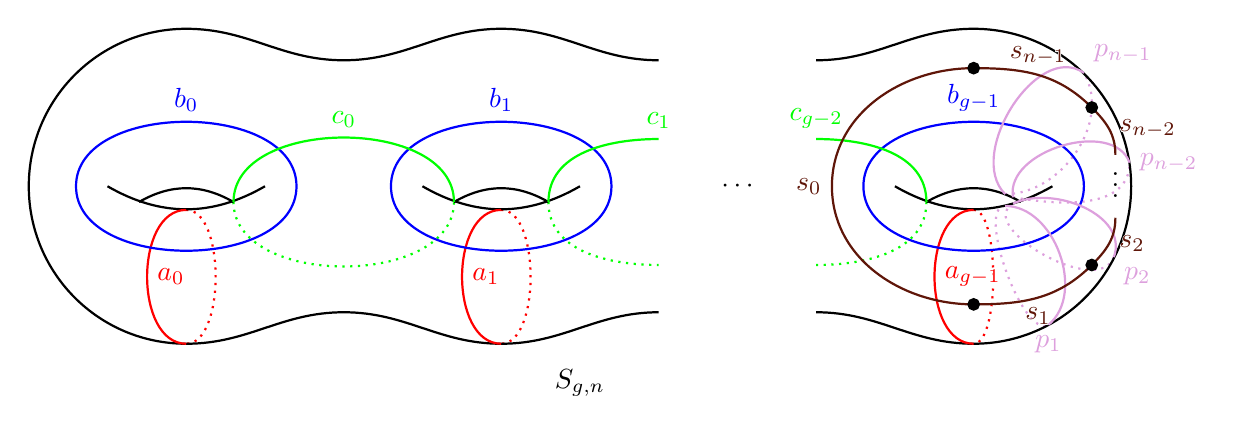
\begin{tikzpicture}[scale=2, thick]
    
    \draw [red, dotted] (-3, -0.15) to [out=0,in=0, looseness=0.75] (-3, -1);
    \draw [red, dotted] (-1, -0.15) to [out=0,in=0, looseness=0.75] (-1, -1);
    \draw [red, dotted] (2, -0.15) to [out=0,in=0, looseness=0.5] (2, -1);
    
    \draw [green, dotted] (-2.7, -0.1) to [out=270,in=270] (-1.3,-0.1);
    \draw [green, dotted] (-0.7, -0.1) to [out=270,in=180] (0,-0.5);
    \draw [green, dotted] (1.7,-0.1) to [out=270,in=0] (1, -0.5);
    
    \draw [Plum, dotted] (2.2, -0.125) to [out=180,in=210, looseness=0.6] (2.475, -0.88);
    \draw [Plum, dotted] (2.25, -0.11) to [out=210,in=250] (2.89, -0.45);
    \draw [Plum, dotted] (2.25, -0.07) to [out=350,in=270] (2.99, 0.15);
    \draw [Plum, dotted] (2.2, -0.05) to [out=0,in=300] (2.7, 0.72);
    
    % Left.
    \draw (0, 0.8)
        to [out=180,in=0] (-1, 1)
        to [out=180,in=0] (-2, 0.8)
        to [out=180,in=0] (-3, 1)
        to [out=180,in=90] (-4, 0)
        to [out=270,in=180] (-3, -1)
        to [out=0,in=180] (-2, -0.8)
        to [out=0,in=180] (-1, -1)
        to [out=0,in=180] (0, -0.8);
    
    % Right.
    \draw (1, 0.8)
        to [out=0,in=180] (2, 1)
        to [out=0,in=90] (3, 0)
        to [out=270,in=0] (2, -1)
        to [out=180,in=0] (1, -0.8);
    
    % Genus.
    \draw (-3.5,0) to [out=-30,in=180+30] (-2.5,0);
    \draw (-3.3,-0.1) to [out=30,in=180-30] (-2.7,-0.1);
    
    \draw (-1.5,0) to [out=-30,in=180+30] (-0.5,0);
    \draw (-1.3,-0.1) to [out=30,in=180-30] (-0.7,-0.1);
    
    \draw (1.5,0) to [out=-30,in=180+30] (2.5,0);
    \draw (1.7,-0.1) to [out=30,in=180-30] (2.3,-0.1);
    
    \node at (0.5, 0) {$\cdots$};
    
    % Front curves:
    % Alpha.
    \draw [red] (-3, -0.15) to [out=180,in=180] node [right] {$a_0$} (-3, -1);
    \draw [red] (-1, -0.15) to [out=180,in=180] node [right] {$a_1$} (-1, -1);
    \draw [red] (2, -0.15) to [out=180,in=180] node [right] {\outline{$a_{g-1}$}} (2, -1);
    
    % Beta.
    \draw [blue] (-3.7, 0) to [out=90,in=90] node [above] {$b_0$} (-2.3, 0) to [out=270,in=270] (-3.7, 0);
    \draw [blue] (-1.7, 0) to [out=90,in=90] node [above] {$b_1$} (-0.3, 0) to [out=270,in=270] (-1.7, 0);
    \draw [blue] (1.3, 0) to [out=90,in=90] node [above] {$b_{g-1}$} (2.7, 0) to [out=270,in=270] (1.3, 0);
    
    % Gamma.
    \draw [green] (-2.7, -0.1) to [out=90,in=90] node [above] {$c_0$} (-1.3,-0.1);
    \draw [green] (-0.7, -0.1) to [out=90,in=180] (0,0.3) node [above] {$c_1$};
    \draw [green] (1.7,-0.1) to [out=90,in=0] (1, 0.3) node [above] {$c_{g-2}$};
    
    % Parallel.
    \draw [Plum] (2.2, -0.125) to [out=0,in=40] (2.475, -0.88) node [below] {$p_1$};
    \draw [Plum] (2.25, -0.11) to [out=25,in=70] (2.89, -0.45) node [below right] {$p_2$};
    \draw [Plum] (2.25, -0.07) to [out=100,in=110] (2.99, 0.15) node [right] {$p_{n-2}$};
    \draw [Plum] (2.2, -0.05) to [out=135,in=145] (2.7, 0.72) node [above right] {$p_{n-1}$};
    
    % Sigma.
    \draw [Sepia] (2.9,0.2)
        to [out=90,in=-45] node [right] {\outline{$s_{n-2}$}} (2.75,0.5)
        to [out=135,in=0] node [above] {\outline{$s_{n-1}$}} (2, 0.75)
        to [out=180,in=90] (1.1, 0) node [left] {\outline{$s_0$}}
        to [out=270,in=180] (2, -0.75)
        to [out=0,in=225] node [below] {\outline{$s_1$}} (2.75, -0.5)
        to [out=45,in=270] node [right] {\outline{$s_2$}} (2.9,-0.2);
    
    % Punctures.
    \node [dot] at (2, -0.75) {};
    \node [dot] at (2.75, -0.5) {};
    \node at (2.9, 0) {$\rvdots$};
    \node [dot] at (2.75, 0.5) {};
    \node [dot] at (2, 0.75) {};
    
    \node at (-0.5, -1.25) {$S_{g,n}$};
\end{tikzpicture}
\end{document}
